\documentclass[11pt,a4paper,fleqn]{article}
\usepackage[english, danish]{babel}
\usepackage[utf8]{inputenc}
\usepackage{amsmath}
% Gør det muligt at inkludere grafik (bl.a. png og jpg) i dokumentet.
\usepackage[pdftex]{graphicx}
\usepackage{tikz}
% Definer hvordan figur tekster ser ud.
\usepackage[textfont={rm, it}, labelfont={bf}]{caption}
% Gør det muligt at medtage flere delfigurer i en enkelt samlet figur.
\usepackage{subfig}
% Aktiverer todonotes pakken
\usepackage{todonotes}
% Gør det muligt at følge henvisninger (links) i dokumentet.
% Beskriver hvordan henvisningerne bliver vist.
\usepackage[colorlinks=true, linkcolor=black, citecolor=black, urlcolor=black]{hyperref}
\usepackage[all]{hypcap}
% Gør det muligt at vise kildekode med syntaks fremhævning i dokumentet.
\usepackage{listings}
\lstset{language=TeX, 
	basicstyle=\footnotesize, 
	tabsize=4,
	numbers=left, 
	numberstyle=\tiny, 
	stepnumber=1, 
	numbersep=5pt}


% ==================================================================
% ============== Setting up fancy headers ... ======================
% ==================================================================
% Holder styr på sidehoved og side fod
\usepackage{fancyhdr}
\pagestyle{fancy}
\renewcommand{\sectionmark}[1]{\markright{\thesection.\ #1}}
\lhead{\korttitel}
\chead{}
\rhead{\rightmark}
\lfoot{\forfattere}
\cfoot{}
\rfoot{\thepage}
\renewcommand{\headrulewidth}{0.5pt}
\renewcommand{\footrulewidth}{0.5pt}


% Øg teksthøjden med 2 cm på alle sider
\addtolength\textheight{2cm}
\addtolength\topmargin{-1cm}
\addtolength\marginparwidth{1.5cm}
\addtolength\headheight{1.6pt}

\makeindex

% ==================================================================
% ============== Various options ===================================
% ==================================================================
\numberwithin{equation}{section}




% ==================================================================
% ============== Indledende oevelser ===============================
% ==================================================================
\title{\titel}
\author{}
\date{}


\newcommand{\forfattere}{Henrik Skov Midtiby}
\newcommand{\titel}{Latex rodebunke med forklaringer}
\newcommand{\korttitel}{Latex rodebunke}
\newcommand{\dato}{2007-12-24}
\newcommand{\fag}{DM63}

\begin{document}


% ==================================================================
% ====== Forside ===================================================
% ==================================================================
\phantom{g}
\vspace{2.5cm}
\noindent
\begin{Huge}
{\titel}
\end{Huge}
\vspace{11cm}

\begin{tabular}{@{} l l @{}}
\hline
Titel           & \titel                \\
Udarbejdet af   & \forfattere           \\
Afleveringsdato & \dato					\\
Fag      		& \fag					\\
\hline
\end{tabular}
\thispagestyle{empty}
\newpage




\tableofcontents
\listoftodos
\newpage


% ==================================================================
% ====== Introduktion ==============================================
% ==================================================================
\section{Introduktion}

I dette dokument vises det hvordan en række forskellige ting kan
gøres i latex. 
\todo{Man kan også indsætte kommentarer i margen om ting der skal 
ændres / forbedres / tjekkes senere.}%
Der er eksempler på hvordan man indsætter en figur, noget kildekode
og meget mere \ldots



\section{Lister}

Latex kan formatere tekst på mange forskellige måder. 
Ofte struktureres ting ved at opstille lister, det kan gøres på denne måde:
%
\begin{lstlisting}
\begin{itemize}
	\item Hund
	\item Elefant
	\item Pindsvin
\end{itemize}
\end{lstlisting}
%
Hvilket givet nedenstående resultat
%
\begin{itemize}
	\item Hund
	\item Elefant
	\item Pindsvin
\end{itemize}
%
Ønsker man en nummereret liste benyttes \emph{enumerate} i stedet for \emph{itemize}.
\todo{Eksempel med lister i lister.}%
Desuden er det muligt at beskrive en række ting
%
\begin{description}
	\item[Æble:] 	En frugt
	\item[Abe:]	Et dyr
\end{description}
%
Koden til det ovenstående er
%
\begin{lstlisting}
\begin{description}
	\item[Banan:] 	En frugt
	\item[Abe:]	Et dyr
\end{description}
\end{lstlisting}





\section{Billeder og figurer}

Billeder indsættes i latex med \verb!\includegraphics! kommandoen.
Ofte ønsker man at angive hvor stort billedet skal være, det gøres 
med \verb!width! og \verb!height! options.

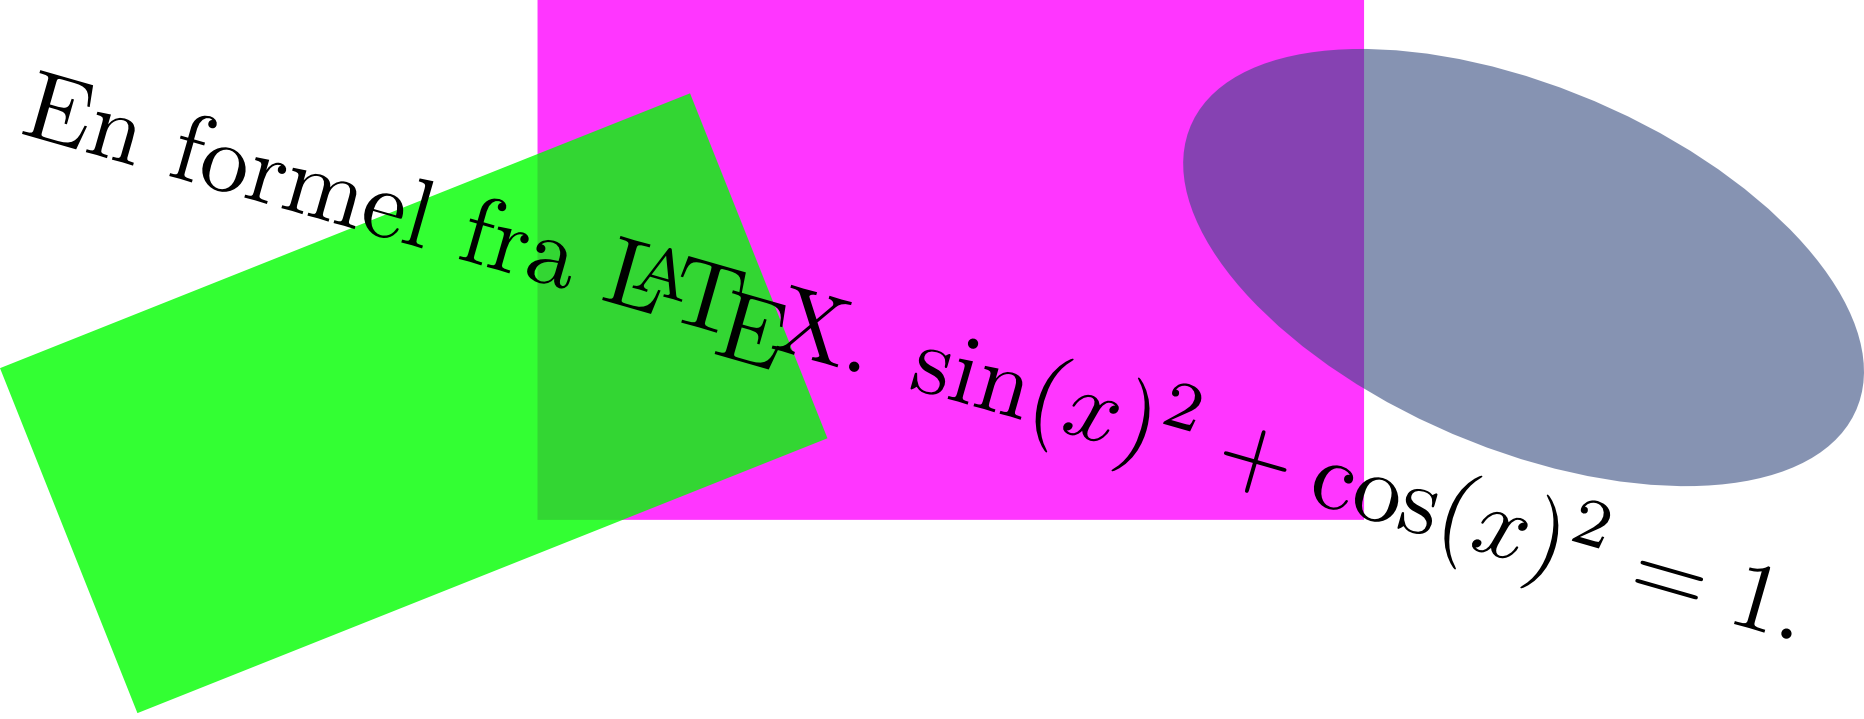
\includegraphics[width=5cm]{pic/figur.png}
\begin{verbatim}
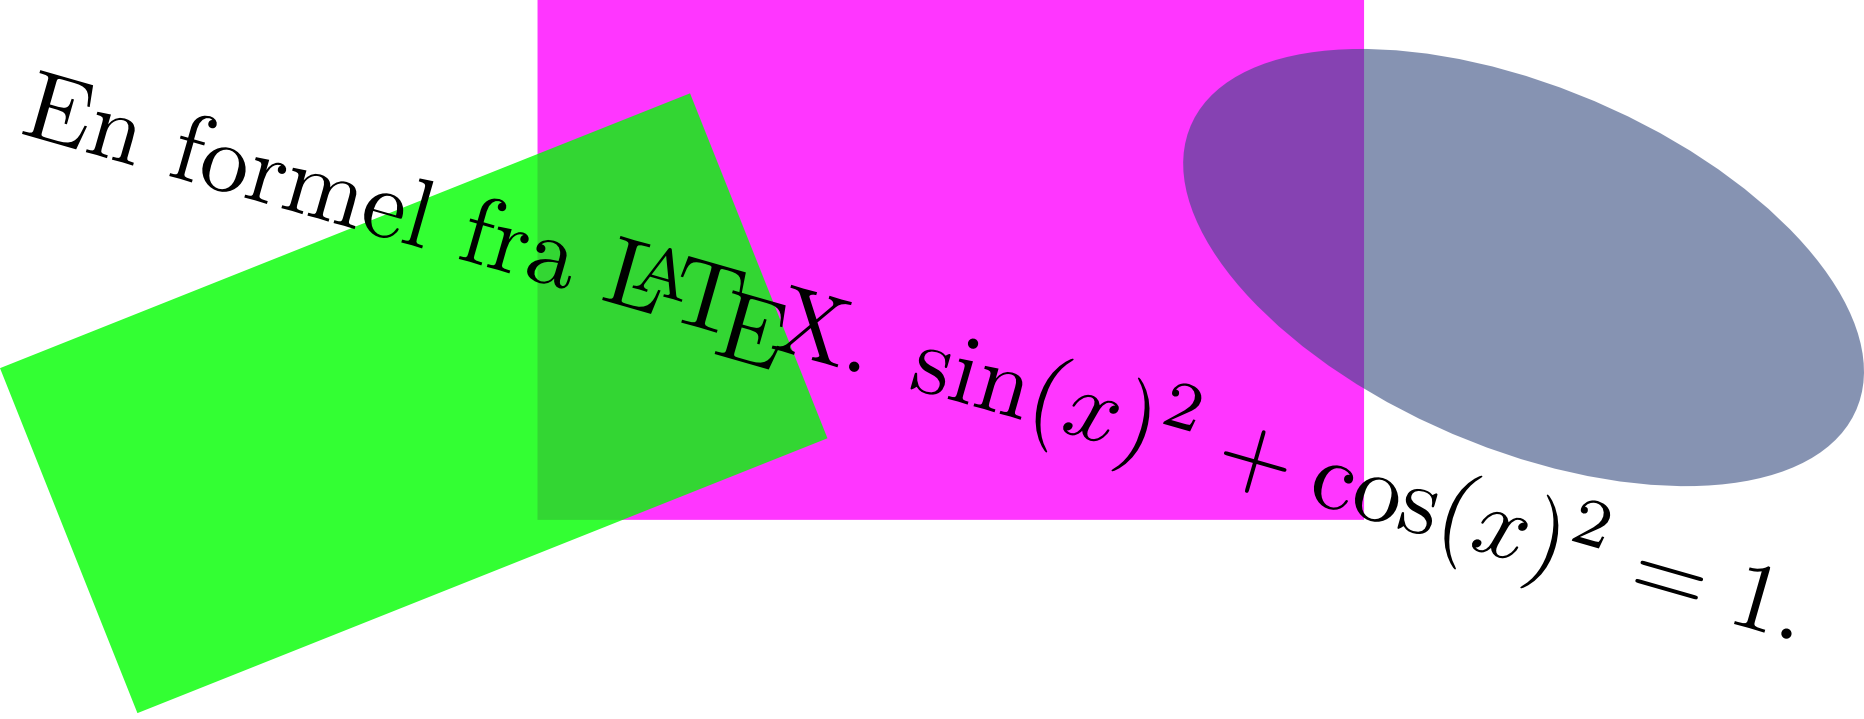
\includegraphics[width=5cm]{pic/figur.png}
\end{verbatim}

Typisk indsættes billeder i et \verb!figure! miljø med tilhørende 
figurnummber og tekst.
Figur \ref{figLabel} er lavet med nedenstående kode:

\begin{verbatim}
\begin{figure}
\centering
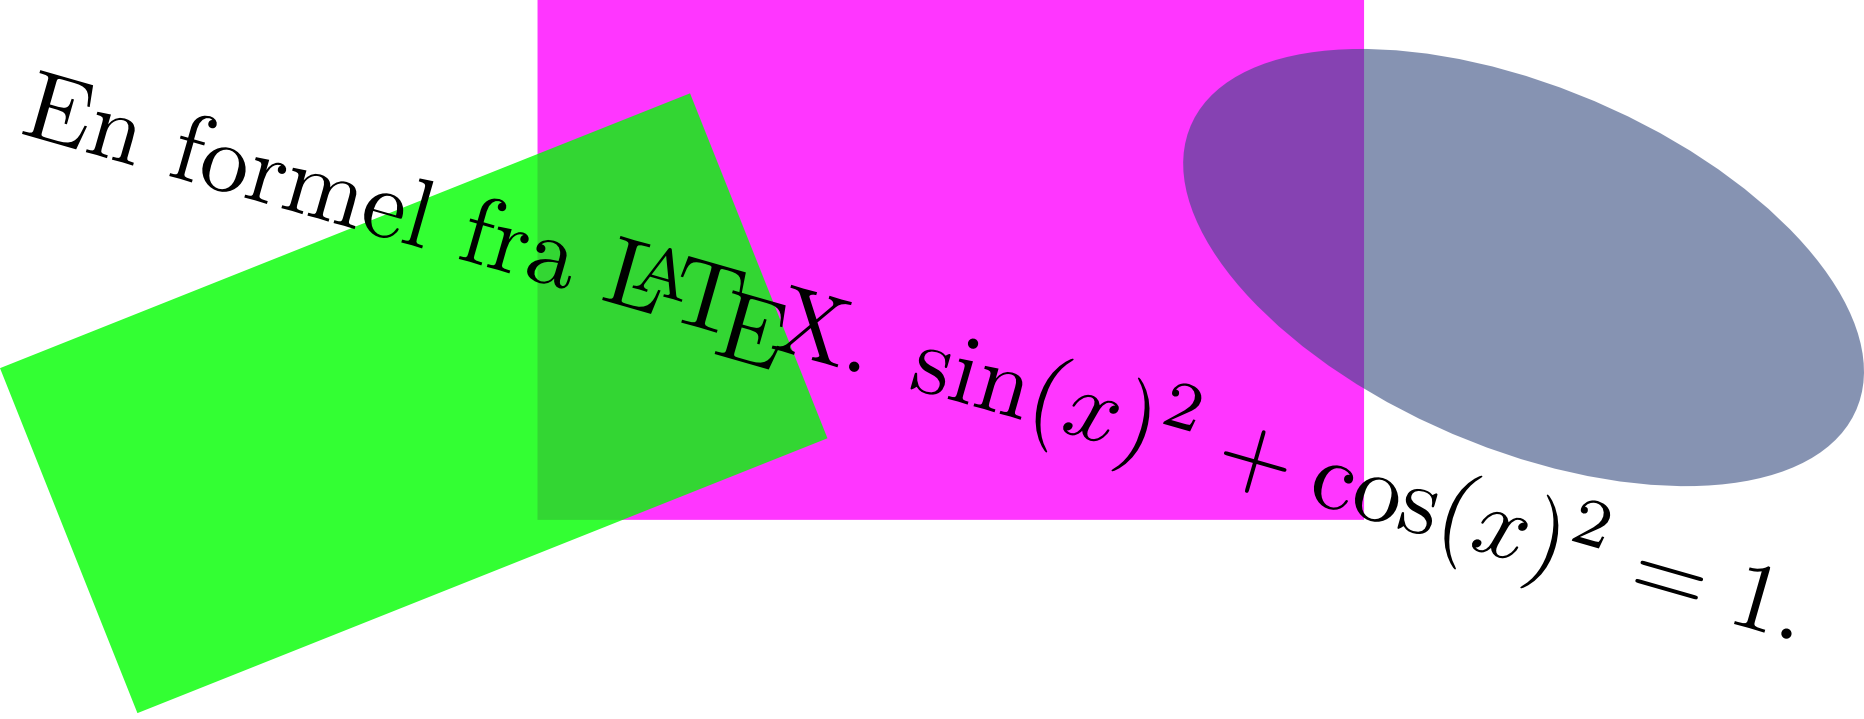
\includegraphics[width=7cm]{pic/figur.png}
\caption{En figurtekst.}
\label{figLabel}
\end{figure}
\end{verbatim}


\begin{figure}
\centering
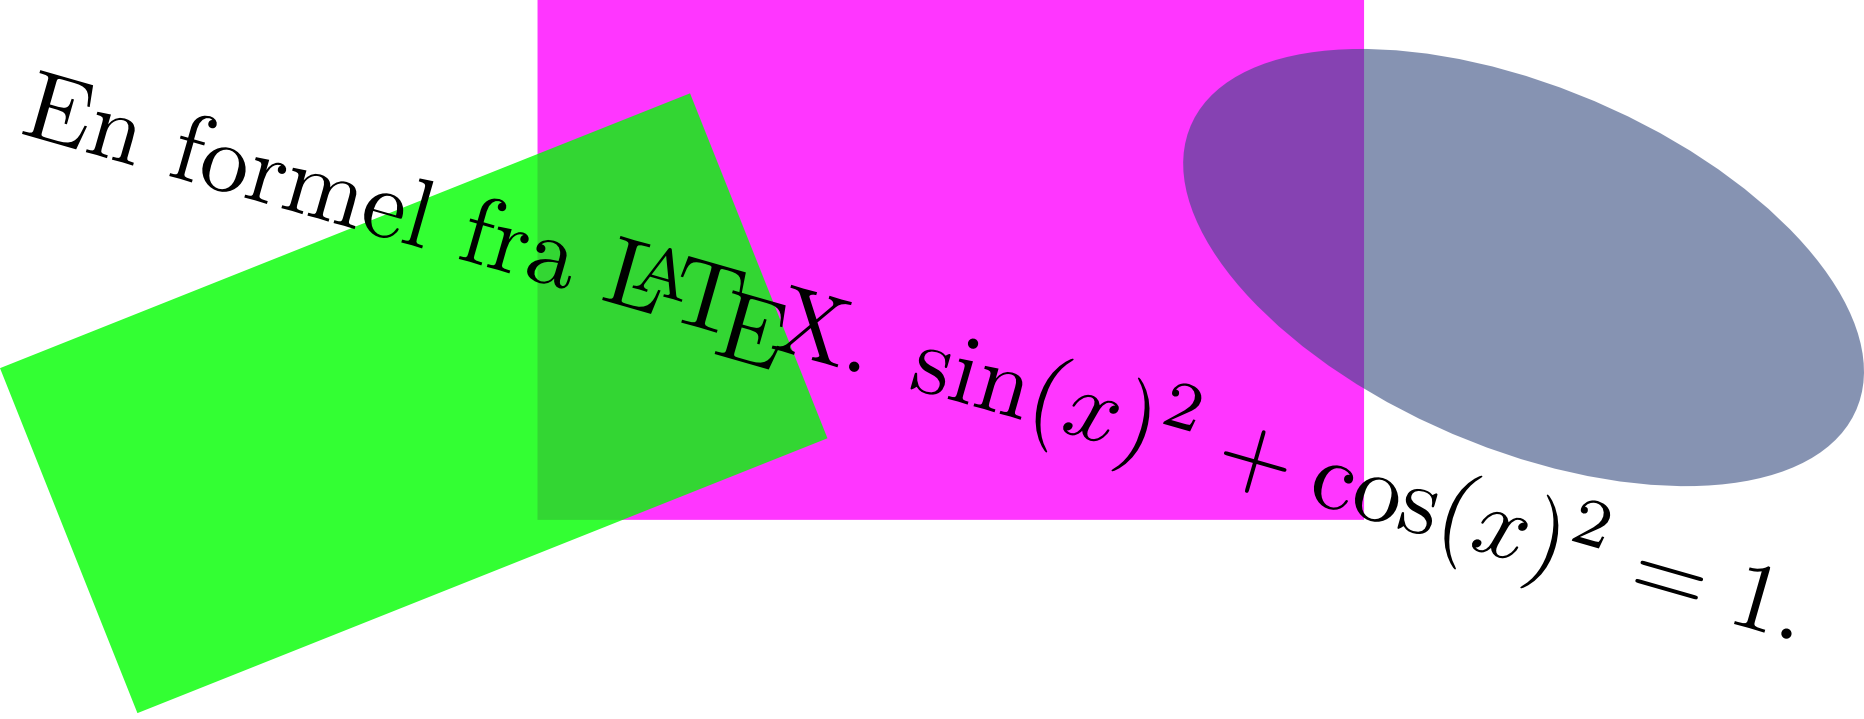
\includegraphics[width=7cm]{pic/figur.png}
\caption{En figurtekst.}
\label{figLabel}
\end{figure}



\section{En figur i TikZ}

PGF/TikZ er et meget kraftfuldt tegnemiljø til \LaTeX .
På \url{http://www.fauskes.net/pgftikzexamples/} er der en stor
samling af eksempler på hvad PGF / TikZ kan præstere.


\subsection{Enhedscirklen med kommentarer}

\begin{tikzpicture}[scale=2.5,cap=round]
  % Local definitions
  \def\costhirty{0.8660256}

  % Colors
  \colorlet{anglecolor}{green!50!black}
  \colorlet{sincolor}{red}
  \colorlet{tancolor}{orange!80!black}
  \colorlet{coscolor}{blue}

  % Styles
  \tikzstyle{axes}=[]
  \tikzstyle{important line}=[very thick]
  \tikzstyle{information text}=[rounded corners,fill=red!10,inner sep=1ex]

  % The graphic
  \draw[style=help lines,step=0.5cm] (-1.4,-1.4) grid (1.4,1.4);

  \draw (0,0) circle (1cm);

  \begin{scope}[style=axes]
    \draw[->] (-1.5,0) -- (1.5,0) node[right] {$x$};
    \draw[->] (0,-1.5) -- (0,1.5) node[above] {$y$};

    \foreach \x/\xtext in {-1, -.5/-\frac{1}{2}, 1}
      \draw[xshift=\x cm] (0pt,1pt) -- (0pt,-1pt) node[below,fill=white]
            {$\xtext$};

    \foreach \y/\ytext in {-1, -.5/-\frac{1}{2}, .5/\frac{1}{2}, 1}
      \draw[yshift=\y cm] (1pt,0pt) -- (-1pt,0pt) node[left,fill=white]
            {$\ytext$};
  \end{scope}

  \filldraw[fill=green!20,draw=anglecolor] (0,0) -- (3mm,0pt) arc(0:30:3mm);
  \draw (15:2mm) node[anglecolor] {$\alpha$};

  \draw[style=important line,sincolor]
    (30:1cm) -- node[left=1pt,fill=white] {$\sin \alpha$} +(0,-.5);

  \draw[style=important line,coscolor]
    (0,0) -- node[below=2pt,fill=white] {$\cos \alpha$} (\costhirty,0);

  \draw[style=important line,tancolor] (1,0) --
    node [right=1pt,fill=white]
    {
      $\displaystyle \tan \alpha \color{black}=
      \frac{{\color{sincolor}\sin \alpha}}{\color{coscolor}\cos \alpha}$
    } (intersection of 0,0--30:1cm and 1,0--1,1) coordinate (t);

  \draw (0,0) -- (t);

  \draw[xshift=2.00cm] node [right,text width=6cm,style=information text]
    {
      The {\color{anglecolor} angle $\alpha$} is $30^\circ$ in the
      example ($\pi/6$ in radians). The {\color{sincolor}sine of
        $\alpha$}, which is the height of the red line, is
      \[
      {\color{sincolor} \sin \alpha} = 1/2.
      \]
      By the Theorem of Pythagoras we have ${\color{coscolor}\cos^2 \alpha} +
      {\color{sincolor}\sin^2\alpha} =1$. Thus the length of the blue
      line, which is the {\color{coscolor}cosine of $\alpha$}, must be
      \[
      {\color{coscolor}\cos\alpha} = \sqrt{1 - 1/4} = \textstyle
      \frac{1}{2} \sqrt 3.
      \]%
      This shows that {\color{tancolor}$\tan \alpha$}, which is the
      height of the orange line, is
      \[
      {\color{tancolor}\tan\alpha} = \frac{{\color{sincolor}\sin
          \alpha}}{\color{coscolor}\cos \alpha} = 1/\sqrt 3.
      \]%
    };
\end{tikzpicture}


\newpage
% ==================================================================
% ====== Forskellige ting ==========================================
% ==================================================================
\section{Forskellige ting}

% ==================================================================
% ==================================================================
\subsection{Styre udseende af figur tekster}

I preamble kan man indstille hvordan figur tekster skal se ud i
dokumentet.
\todo{En ting jeg gerne vil have ændret i dokumentet.}%
Det gøres ved at inkludere pakken \verb!caption! og give den en
række argumenter.
F.eks. giver følgende figur tekster hvor figur nummeret står med en
ikke kursiv fed tekst og resten af figur teksten står i
kursiv.
%
\begin{lstlisting}
\usepackage[textfont={rm, it}, labelfont={bf}]{caption}
\end{lstlisting}


% ==================================================================
% ==================================================================
\subsection{Interne links i dokumenter}

Når pakken \verb!hyperref! inkluderes i preamblet vil latex lave
henvisninger i dokumentet om til links, som læseren kan følge når
\todo{Noget der skal ændres i dokumentet.}%
dokumentet læses.
%
\begin{lstlisting}
\usepackage{hyperref}
\end{lstlisting}
%
Hvis man ikke ønsker kasser omkring de dannede links (som det gøres
pr. default) kan ovenstående linie erstattes med følgende
%
\begin{lstlisting}
\usepackage[colorlinks=true, linkcolor=black, 
            citecolor=black, urlcolor=black]{hyperref}
\end{lstlisting}
%
ønsker man at linkene skiller sig ud fra den omgivende tekst, kan
\verb!black! udskiftes med f.eks. \verb!red! og linkene bliver i så
fald røde.


% ==================================================================
% ==================================================================
\subsection{Sidehoved og sidefod}

Pakken \verb!fancyhdr!, gør det muligt at indsætte sidehoved og
sidefod på sine dokumenter.
%
\begin{lstlisting}
\usepackage{fancyhdr}
\end{lstlisting}
%
Udseendet af sidehovedet og sidefoden defineres ved følgende række
kommandoer, som regel er placeret i preamblet.
%
\begin{lstlisting}
\pagestyle{fancy}
\lhead{\korttitel}
\chead{}
\rhead{\rightmark}
\lfoot{\forfattere}
\cfoot{}
\rfoot{\thepage}
\renewcommand{\headrulewidth}{0.5pt}
\renewcommand{\footrulewidth}{0.5pt}
\end{lstlisting}
%
Ovenstående kode, er den der er benyttet til at generere sidehovedet
og foden på dette dokument.

\subsection{Skrive matematik}

Jeg benytter pakken \verb!amsmath! til at sætte formler op i. 
Den giver mulighed for at skrive mellem regninger pænt under
hinanden (sådan at alle lighedstegn står over / under hinanden).
%
\begin{lstlisting}
\usepackage{amsmath}
\end{lstlisting}
%
Herunder er der nogle eksempler på hvordan matematikken kan se ud og
hvordan det skrives.
Først idiot formlen.
%
\begin{align*}
1
	& = \sin(x)^2 + \cos(x)^2 
\end{align*}
%
\begin{lstlisting}
\begin{align*}
1
	& = \sin(x)^2 + \cos(x)^2 
\end{align*}
\end{lstlisting}
%
Så Schrödinger ligningen i et endimensionelt system 
%
\begin{align}
\left(\frac{-\hbar^2}{2m} \frac{\partial^2}{\partial x^2} 
		+ V(x)\right) \Psi(t, x)
	& = E \Psi(t, x)
\end{align}
%
Koden er så
%
\begin{lstlisting}
\begin{align}
\left(\frac{-\hbar^2}{2m} \frac{\partial^2}{\partial x^2} 
		+ V(x)\right) \Psi(t, x)
	& = E \Psi(t, x)
\end{align}
\end{lstlisting}
%
Har man behov for at forklare hvad de enkelte dele af en formel
betyder, kan det gøres med 
\verb!\underbrace{formel del}_{forklaring}! kommandoen.
%
\begin{align}
\nonumber
\underbrace{\left(\underbrace{\frac{-\hbar^2}{2m} 
		\frac{\partial^2}{\partial x^2}}_{\textrm{Kinetisk energi}} 
		+ \underbrace{V(x)}_{\textrm{Potentiel energi}}
		\right)}_{\textrm{Hamilton operator}}
		\underbrace{\Psi(t, x)}_{\textrm{Bølgefunktion}}
	& = \underbrace{E}_{\textrm{Systemets energi}} \Psi(t, x)
\end{align}
%
\begin{lstlisting}
\begin{align}
\nonumber
\underbrace{\left(\underbrace{\frac{-\hbar^2}{2m} 
		\frac{\partial^2}{\partial x^2}}_{\textrm{Kinetisk energi}} 
		+ \underbrace{V(x)}_{\textrm{Potentiel energi}}
		\right)}_{\textrm{Hamilton operator}}
		\underbrace{\Psi(t, x)}_{\textrm{Blgefunktion}}
	& = \underbrace{E}_{\textrm{Systemets energi}} \Psi(t, x)
\end{align}
\end{lstlisting}



% ==================================================================
% ==================================================================
% ==================================================================
\end{document}

